\documentclass[10pt,a4paper,twocolumn]{article}

% Page geometry to match the conference template
\usepackage[top=2.5cm,right=2.0cm,bottom=3.0cm,left=3.0cm]{geometry}
\setlength{\columnsep}{1cm}

% Fonts and text settings
\usepackage[T1]{fontenc}
\usepackage{mathptmx}
\usepackage[utf8]{inputenc}
\linespread{1}
\setlength{\parindent}{0.5cm}
\pagestyle{empty}

% Mathematics and utilities
\usepackage{amsmath}
\usepackage{graphicx}
\usepackage{booktabs}
\usepackage{array}

% Figures and captions in 9 pt
\usepackage[font=small,labelfont=bf]{caption}
\captionsetup[figure]{font=small,justification=centering,skip=5pt}
\captionsetup[table]{font=small,justification=centering,skip=5pt}

% Harvard style citations
\usepackage{natbib}
\setcitestyle{authoryear,open={(},close={)},semicolon={;},aysep={,},yysep={,}}
\renewcommand{\refname}{\centering References}

% TikZ for the required graphs
\usepackage{tikz}
\usetikzlibrary{shapes.geometric,arrows.meta,positioning,calc}
\usepackage{pgfplots}
\pgfplotsset{compat=1.17}

\begin{document}

% Title block spanning both columns
\twocolumn[{
\begin{center}
{\LARGE\bfseries PLC Based Multi Sensor Condition Monitoring of Industrial Motors for Industrial Transformation\\[6pt]}
{\large TAKUNDA PAMBAYI\textsuperscript{*} \hspace{1.5cm} ENG TANAKA D DZAPASI\textsuperscript{**}\\[2pt]}
{\normalsize Harare Institute of Technology, Harare, Zimbabwe\\[6pt]}
\end{center}

\noindent\textbf{Abstract.} Industrial motors drive pumps, compressors, fans and conveyors. Unexpected failure stops production. This paper presents a practical condition monitoring framework that uses a programmable logic controller to combine motor electrical current and mechanical vibration. Time and frequency domain features are fused to classify normal, warning and critical states. The work suits plants that already have PLC infrastructure and need an affordable step from preventive to condition based maintenance.\\[3pt]
\textbf{Key words:} PLC, condition monitoring, induction motor, multi sensor fusion, predictive maintenance.\\[3pt]
\small\textbf{Address for correspondence:} Takunda Pambayi, Harare Institute of Technology, Ganges Road, Harare, Zimbabwe; e-mail: tpambayi@hit.ac.zw
\vspace{6pt}
}]

\section*{Introduction}
Electric motors keep factories moving. When one fails, an entire process line can stop. Conventional maintenance often runs on fixed calendars or waits for visible trouble. Both approaches miss early signs and can waste spare parts.

Condition based maintenance uses live measurements to decide when attention is needed. Current can be measured without touching the rotating shaft \citep{benbouzid2000}. Vibration gives direct evidence of mechanical wear, imbalance and looseness \citep{gangsar2020}. Many plants already use programmable logic controllers for motor control, so adding condition logic to the same PLC keeps monitoring affordable.

This paper proposes a PLC based multi sensor system for industrial induction motors. It combines electrical current and vibration evidence to detect abnormal states early.

\section*{Related Work and Research Gap}
Motor current signature analysis identifies abnormal patterns in stator current spectra \citep{benbouzid2000}. Vibration analysis captures bearing defects, misalignment and looseness \citep{gangsar2020}. \citet{yang2006} showed that combining the two signals improves fault decisions. Recent work has extended these methods to variable speed drives \citep{niu2023,yakhni2023}. Many advanced systems, however, still need specialist hardware or machine learning platforms that smaller factories cannot afford. The gap is a transparent, PLC centred method that fits existing control infrastructure.

\section*{Proposed System Architecture}
The system has five layers: sensing, signal conditioning, feature extraction, PLC decision and HMI visualization. Current transformers and accelerometers collect signals. Filters and isolators condition them. The PLC compares extracted features against thresholds and fuses them. Sensor mounting matters; the accelerometer should sit near the bearing in a fixed radial direction, and operating speed, load and sampling settings must be logged \citep{iso2016}.

\begin{figure}[htbp]
\centering
\small
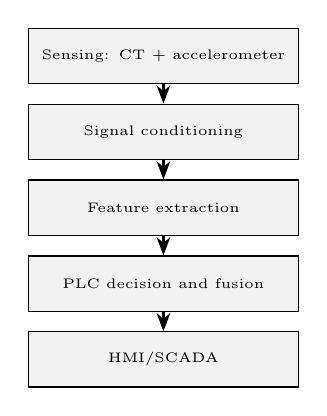
\begin{tikzpicture}[
    node distance=0.25cm,
    box/.style={rectangle, draw, fill=gray!10, text width=3.2cm, align=center, font=\tiny, minimum height=0.7cm},
    arrow/.style={-Stealth, thick}
]
\node[box] (s) {Sensing: CT + accelerometer};
\node[box, below=of s] (c) {Signal conditioning};
\node[box, below=of c] (f) {Feature extraction};
\node[box, below=of f] (p) {PLC decision and fusion};
\node[box, below=of p] (h) {HMI/SCADA};
\draw[arrow] (s) -- (c);
\draw[arrow] (c) -- (f);
\draw[arrow] (f) -- (p);
\draw[arrow] (p) -- (h);
\end{tikzpicture}
\caption{Proposed PLC based multi sensor monitoring architecture.}
\label{fig:architecture}
\end{figure}

\section*{Signal Processing and Fusion}
For a sampled current window of $N$ samples, the RMS current is
\begin{equation}
I_{\mathrm{RMS}} = \sqrt{\frac{1}{N}\sum_{k=1}^{N} i_k^2}.
\label{eq:irms}
\end{equation}
Three phase imbalance is the largest phase deviation from the average current divided by the average. Vibration RMS is computed similarly, while crest factor links peak acceleration to RMS vibration:
\begin{equation}
\mathrm{Crest\;Factor} = \frac{\max(|x_k|)}{X_{\mathrm{RMS}}}.
\label{eq:crest}
\end{equation}
Spectral features come from the Fast Fourier Transform, with bin spacing $\Delta f = F_s/N$.

Each feature is normalised against a healthy baseline. The electrical indicator $C$ and vibration indicator $V$ are clipped to $[0,1]$. A weighted fusion score then combines them:
\begin{equation}
S = w_c C + w_v V,\quad w_c + w_v = 1.
\label{eq:fusion}
\end{equation}
If $C=0.65$, $V=0.85$, $w_c=0.40$ and $w_v=0.60$, then $S=0.77$, which falls in the warning band when warning and critical thresholds are $0.60$ and $0.80$.

\begin{figure}[htbp]
\centering
\small
\resizebox{\columnwidth}{!}{%
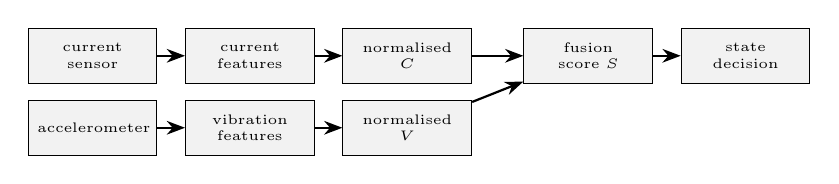
\begin{tikzpicture}[
    node distance=0.2cm and 0.35cm,
    box/.style={rectangle, draw, fill=gray!10, text width=1.4cm, align=center, font=\tiny, minimum height=0.7cm},
    arrow/.style={-Stealth, thick}
]
\node[box] (ct) {current sensor};
\node[box, right=of ct] (cf) {current features};
\node[box, right=of cf] (cn) {normalised $C$};
\node[box, below=of ct] (acc) {accelerometer};
\node[box, right=of acc] (vf) {vibration features};
\node[box, right=of vf] (vn) {normalised $V$};
\node[box, right=of cn, xshift=0.3cm] (fuse) {fusion score $S$};
\node[box, right=of fuse] (dec) {state decision};
\draw[arrow] (ct) -- (cf);
\draw[arrow] (cf) -- (cn);
\draw[arrow] (acc) -- (vf);
\draw[arrow] (vf) -- (vn);
\draw[arrow] (cn) -- (fuse);
\draw[arrow] (vn) -- (fuse);
\draw[arrow] (fuse) -- (dec);
\end{tikzpicture}%
}
\caption{Signal processing and fusion chain from sensors to PLC decision.}
\label{fig:processing}
\end{figure}

\section*{PLC Decision and HMI}
The PLC assigns one of four states. Normal means all features are within healthy limits. Warning means one feature has crossed its warning threshold for a persistence period. Critical means several features are abnormal or a severe threshold is passed. Sensor fault flags missing or saturated readings so the system does not decide from bad data. The HMI shows motor status, current and vibration RMS, condition state, alarm history and sensor health.

\begin{table}[htbp]
\centering
\scriptsize
\caption{Expected indicator behaviour for selected conditions.}
\label{tab:conditions}
\begin{tabular}{>{\raggedright\arraybackslash}p{1.4cm}>{\raggedright\arraybackslash}p{2.4cm}>{\raggedright\arraybackslash}p{2.4cm}}
\toprule
Condition & Current evidence & Vibration evidence \\
\midrule
Healthy & Stable RMS and spectrum & Stable RMS and spectrum \\
Overload & High RMS current & Load related increase \\
Bearing wear & Modulation sidebands & RMS, crest factor and kurtosis rise \\
Misalignment & Current variation & Axial/radial vibration increase \\
Electrical fault & Imbalance or distortion & Secondary response \\
\bottomrule
\end{tabular}
\end{table}

\section*{Validation and Discussion}
Validation should start with healthy data at several loads. Controlled faults such as imbalance or misalignment are then introduced one at a time. Metrics include detection rate, false alarm rate, detection latency and monitoring availability \citep{iec2026}. Figure \ref{fig:comparison} compares the proposed fused approach with current only and vibration only monitoring. The fused approach scores higher on both electrical and mechanical sensitivity. The main benefit is earlier warning without a separate specialist system. Limitations include motor specific baselines and the effects of sensor mounting, VFD switching and load variation.

\begin{figure}[htbp]
\centering
\footnotesize
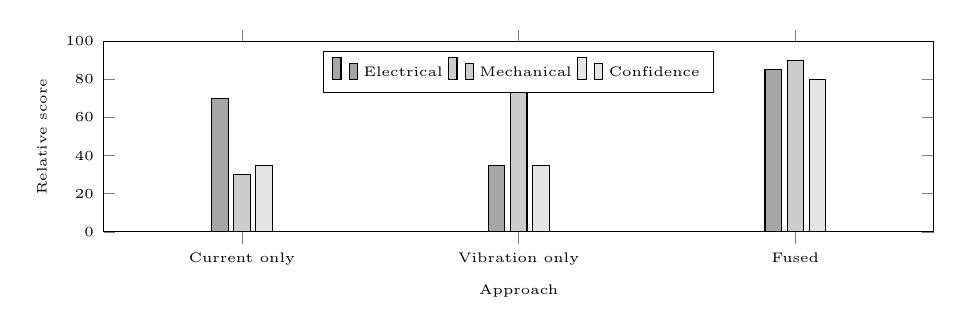
\begin{tikzpicture}
\begin{axis}[
    ybar,
    width=\columnwidth,
    height=4cm,
    bar width=6pt,
    ylabel={Relative score},
    ylabel style={font=\tiny},
    xlabel={Approach},
    xlabel style={font=\tiny},
    symbolic x coords={Current only, Vibration only, Fused},
    xtick=data,
    xticklabel style={font=\tiny},
    yticklabel style={font=\tiny},
    ymin=0, ymax=100,
    legend style={font=\tiny, at={(0.5,0.95)}, anchor=north, legend columns=3},
    enlarge x limits=0.25,
]
\addplot[fill=gray!70] coordinates {(Current only,70) (Vibration only,35) (Fused,85)};
\addplot[fill=gray!40] coordinates {(Current only,30) (Vibration only,80) (Fused,90)};
\addplot[fill=gray!20] coordinates {(Current only,35) (Vibration only,35) (Fused,80)};
\legend{Electrical, Mechanical, Confidence}
\end{axis}
\end{tikzpicture}
\caption{Illustrative comparison of monitoring strategies. Values are not measured data.}
\label{fig:comparison}
\end{figure}

\section*{Conclusion}
A PLC based multi sensor framework for industrial motor condition monitoring has been presented. It combines current and vibration evidence into transparent indicators and fuses them through simple PLC logic. The design uses existing automation infrastructure, making it accessible to factories that cannot yet invest in advanced analytics platforms. Future work should validate thresholds on a motor test rig and extend the system with temperature, voltage and speed information.

\begin{footnotesize}\raggedright
\setlength{\bibsep}{0pt}
\begin{thebibliography}{99}
\bibitem[Benbouzid(2000)]{benbouzid2000} Benbouzid, M.E.H. (2000) `A review of induction motors signature analysis as a medium for faults detection', \textit{IEEE Transactions on Industrial Electronics}, 47(5), pp. 984--993. doi:10.1109/41.873206.
\bibitem[Gangsar and Tiwari(2020)]{gangsar2020} Gangsar, P. and Tiwari, R. (2020) `Signal based condition monitoring techniques for fault detection and diagnosis of induction motors: a state of the art review', \textit{Mechanical Systems and Signal Processing}, 144, p. 106908. doi:10.1016/j.ymssp.2020.106908.
\bibitem[Yang and Kim(2006)]{yang2006} Yang, B.S. and Kim, K.J. (2006) `Application of Dempster--Shafer theory in fault diagnosis of induction motors using vibration and current signals', \textit{Mechanical Systems and Signal Processing}, 20(2), pp. 403--420. doi:10.1016/j.ymssp.2004.10.010.
\bibitem[Niu(2023)]{niu2023} Niu, G. (2023) `Motor fault diagnostics based on current signatures: a review', \textit{IEEE Transactions on Instrumentation and Measurement}, 72, p. 3520919. doi:10.1109/TIM.2023.3285999.
\bibitem[Yakhni et al.(2023)]{yakhni2023} Yakhni, M.F., Cauet, S., Sakout, A., Assoum, H., Etien, E., Rambault, L. and El Gohary, M. (2023) `Variable speed induction motors' fault detection based on transient motor current signatures analysis: a review', \textit{Mechanical Systems and Signal Processing}, 184, p. 109737. doi:10.1016/j.ymssp.2022.109737.
\bibitem[ISO(2016)]{iso2016} ISO (2016) \textit{ISO 20816-1:2016 Mechanical vibration -- Measurement and evaluation of machine vibration -- Part 1: General guidelines}. Geneva: International Organization for Standardization.
\bibitem[IEC(2026)]{iec2026} IEC (2026) \textit{IEC 60034-1:2026 Rotating electrical machines -- Part 1: Rating and performance}. Geneva: International Electrotechnical Commission.
\end{thebibliography}
\end{footnotesize}

\end{document}
